\chapter{Other compositions}
\label{sec:comps}

Up until this point we have looked in detail at the high-entropy silicide \ch{(CrFeMnNi)Si2} and associated SQSs. However these structures are just the center of a quaternary phase diagram consisting of the different possible distributions of elements Thus there exists many other possible compositions related to the previosuly explored \ch{(CrFeMnNi)Si2} high-entropy silicide. In the two following sections we will analyze some of the different possibilities, starting with a discussion on alloys based on the same elements but with different distributions. Thereafter we will look at alloys where chromium, manganese or nickel are replaced with cobalt or titanium. 

\section{Exploring the quaternary phase-diagram}
In this section, we aim to expand our search of this diagram by generating SQSs of the 48 atom model slightly away from equimolar distribution of 3d elements. In table (bellow) we list the mean total energy and magnetic moment per atom with standard deviation and the enthalpy of formation of 4 compositions of the \ch{(CrFeMnNi)Si2} alloy. Ideally they would differ only by one element, but the TDEP implementation insist in also reducing Nickel to stay consistent with the 48 atom supercell, therfore we include a composition with solely larger amounts of nickel as well. 

\begin{table}[H]
\centering
\begin{tabular}{@{}cccccc@{}}
\toprule
Composition           & \multicolumn{2}{c}{\begin{tabular}[c]{@{}c@{}}Toten\\ (eV)\end{tabular}} & \multicolumn{2}{c}{\begin{tabular}[c]{@{}c@{}}Mag \\ ($\mu_B$) \end{tabular}} & \begin{tabular}[c]{@{}c@{}}$E_{FPA}$\\ (eV) \end{tabular} \\ \midrule
                      & mean                                 & std                               & mean                                 & std                                 & mean                                                      \\ \midrule
\ch{Cr3Fe3Mn7Ni3Si32} & - 6.6947                             & 0.0040                            & 0.1375                               & 0.0186                              & -0.300                                                  \\
\ch{Cr5Fe5Mn3Ni3Si32} & - 6.6705                             & 0.0030                            & 0.1127                               & 0.0223                              & -0.286                                                  \\
\ch{Cr5Fe3Mn5Ni3Si32} & - 6.6852                             & 0.0041                            & 0.1375                               & 0.0456                              & -0.271                                                  \\
\ch{Cr3Fe5Mn5Ni3Si32} & - 6.6801                             & 0.0036                            & 0.0937                               & 0.0209                              & -0.315                                                  \\
\ch{Cr3Fe3Mn3Ni7Si32} & - 6.3921                             & 0.0078                            & 0.0159                               & 0.0101                              & -0.285                                                  \\ \bottomrule
\end{tabular}
\caption{Summary composition diagram}
\end{table}

In table 8.1 we observe that moving away from the equimolar system generally result in lesser stable compositions, with the immense exception of compositions rich in nickel. Here we find that the formation energy is about twice the amount of the other compositions and additionally exceeds the equimolar system. The physical reason behind why nickel have such a large effect on the enthalpy of formation is beyond the scope of this study, but we do note that we have not found any indication of nickel stabilizing high-entropy alloys or silicides, but in terms of mathematics it's sensible that $\delta H$ is larger from the low total energy of nickel ($5.58 eV$) compared to for example Cr ($9.51 eV$) or Mn ($9.03$). 

  
Compared to the equimolar system, the magnetic moment of these compositions show a greater variation between SQSs, as indicated by the standard deviation. Typically the most stable SQS lie around the mean value of the set. The large magnetic moment of the manganese rich permutation and the low magnetic moment in the chromium poor permutation is very much in line with the observations made in the previous section. Recalling that in the magnetic moment in the equimolar composition was largely attributed to manganese and chromium atoms in the lattice. Thus increments to manganese or reduction of chromium would following impact the magnetic moment as seen. Following the composition \ch{Cr5Fe3Mn5Ni3Si32} where the nonmagnetic elements are reduced and the magnetic elements are increased, the final magnetic moment is among the highest of the bunch equally magnetic. 

In table 8.2 we list the respective band gaps of the different compositions calculated with the PBE functional. Only the GGA functional was applied in this case because the motivation is primarily to compare the results to the parent equimolar composition and thus including 3 times as many results to calculate and analyze unnecessarily complicate the process. Thus we base this comparison between the PBE results of the new compositions to the PBE band gaps of the equimolar compound. In these compositions we find strong indication of a half-metal with less frequent SQSs with a band gap in the spin down channel than the equimolar compound. In the spin up channel on the other hand several compositions show very similar values to the equimolar composition. Between the different compositions particularly those rich in manganese provide very encouraging results and compositions poor in Mn less so. In terms of the stability we a very encouraging results of both the \ch{Cr3Fe3Mn7Ni3Si32} and \ch{Cr3Fe5Mn5Ni3Si32} compositions, where the most promising properties is attributed to the utmost stable configurations.  in \ch{Cr3Fe5Mn5Ni3Si32} the most stable SQS (D) is a semiconductor with a band gap around 0.1 eV.

\begin{table}[H]
\centering
\begin{tabular}{@{}ccccc@{}}
\toprule
Composition                                                 & SQS        & \begin{tabular}[c]{@{}c@{}}$E_G ^\text{up, eigen}(0.5)$\\ (eV)\end{tabular} & \begin{tabular}[c]{@{}c@{}}$E_G ^\text{dw, eigen}(0.5)$\\ (eV)\end{tabular} & \begin{tabular}[c]{@{}c@{}}$E_G ^\text{tot, eigen}(0.5, 0.5)$\\ (eV)\end{tabular} \\ \midrule
\multicolumn{1}{c|}{\multirow{5}{*}{\ch{Cr3Fe3Mn7Ni3Si32}}} & A          & 0.3390                                                                      & 0                                                                           & 0                                                                                 \\
\multicolumn{1}{c|}{}                                       & \textbf{B} & 0.4745                                                                      & 0                                                                           & 0                                                                                 \\
\multicolumn{1}{c|}{}                                       & C          & 0.1342                                                                      & 0                                                                           & 0                                                                                 \\
\multicolumn{1}{c|}{}                                       & D          & 0.1950                                                                      & 0.0063                                                                      & 0.0063                                                                            \\
\multicolumn{1}{c|}{}                                       & E          & 0.4211                                                                      & 0                                                                           & 0                                                                                 \\ \midrule
\multicolumn{1}{c|}{\multirow{4}{*}{\ch{Cr5Fe5Mn3Ni3Si32}}} & A          & \textit{0.003}                                                              & 0                                                                           & 0                                                                                 \\
\multicolumn{1}{c|}{}                                       & \textbf{C} & \textit{0.21}                                                               & 0                                                                           & 0                                                                                 \\
\multicolumn{1}{c|}{}                                       & D          & 0.0674                                                                      & 0.0413                                                                      & 0.0372                                                                            \\
\multicolumn{1}{c|}{}                                       & E          & \textit{0.362}                                                              & 0                                                                           & 0                                                                                 \\ \midrule
\multicolumn{1}{c|}{\multirow{5}{*}{\ch{Cr5Fe3Mn5Ni3Si32}}} & \textbf{A} & 0.2082                                                                      & 0                                                                           & 0                                                                                 \\
\multicolumn{1}{c|}{}                                       & B          & 0.4053                                                                      & 0                                                                           & 0                                                                                 \\
\multicolumn{1}{c|}{}                                       & C          & 0.4659                                                                      & 0                                                                           & 0                                                                                 \\
\multicolumn{1}{c|}{}                                       & D          & 0.0843                                                                      & 0.0121                                                                      & 0.0121                                                                            \\
\multicolumn{1}{c|}{}                                       & E          & 0.3008                                                                      & 0                                                                           & 0                                                                                 \\ \midrule
\multicolumn{1}{c|}{\multirow{4}{*}{\ch{Cr3Fe5Mn5Ni3Si32}}} & A          & 0.3922                                                                      & 0                                                                           & 0                                                                                 \\
\multicolumn{1}{c|}{}                                       & C          & 0.1285                                                                      & 0                                                                           & 0                                                                                 \\
\multicolumn{1}{c|}{}                                       & \textbf{D} & 0.2595                                                                      & 0.1004                                                                      & 0.1004                                                                            \\
\multicolumn{1}{c|}{}                                       & E          & 0.3591                                                                      & 0.1003                                                                      & 0.0848                                                                            \\ \midrule
\multicolumn{1}{c|}{\multirow{5}{*}{{Cr3Fe3Mn3Ni7Si32}}}    & A          & 0                                                                           & 0                                                                           & 0                                                                                 \\
\multicolumn{1}{c|}{}                                       & B          & 0                                                                           & 0                                                                           & 0                                                                                 \\
\multicolumn{1}{c|}{}                                       & C          & 0                                                                           & 0                                                                           & 0                                                                                 \\
\multicolumn{1}{c|}{}                                       & D          & 0                                                                           & 0                                                                           & 0                                                                                 \\
\multicolumn{1}{c|}{}                                       & \textbf{E} & \textit{0.04}                                                               & 0                                                                           & 0                                                                                 \\ \bottomrule 
\end{tabular}
\caption{Band gaps of various compositions of \ch{(CrFeMnNi)Si2}. Most stable SQS of a set is highlighted in bold text, defect band gap are listed in cursive. Some SQSs were excluded from the table due to unsuccessful calculations.}
\end{table}

Below in figure 8.1 we plot the projected density of states around $E_F$ of the fist four compositions of table 8.2. Note that away from the Fermi energy the projected density of states is analogous to the parent equimolar composition. The below figures is based on the most stable SQS in each permutation, as will the analysis. Hence the features of these figures can be subject to the uniqueness of that particular SQS rather than a distinct feature of the exact composition, but as stated previously the most stable configuration provide the most likely properties of the composition within the scope of this project. 

\begin{figure}[H]
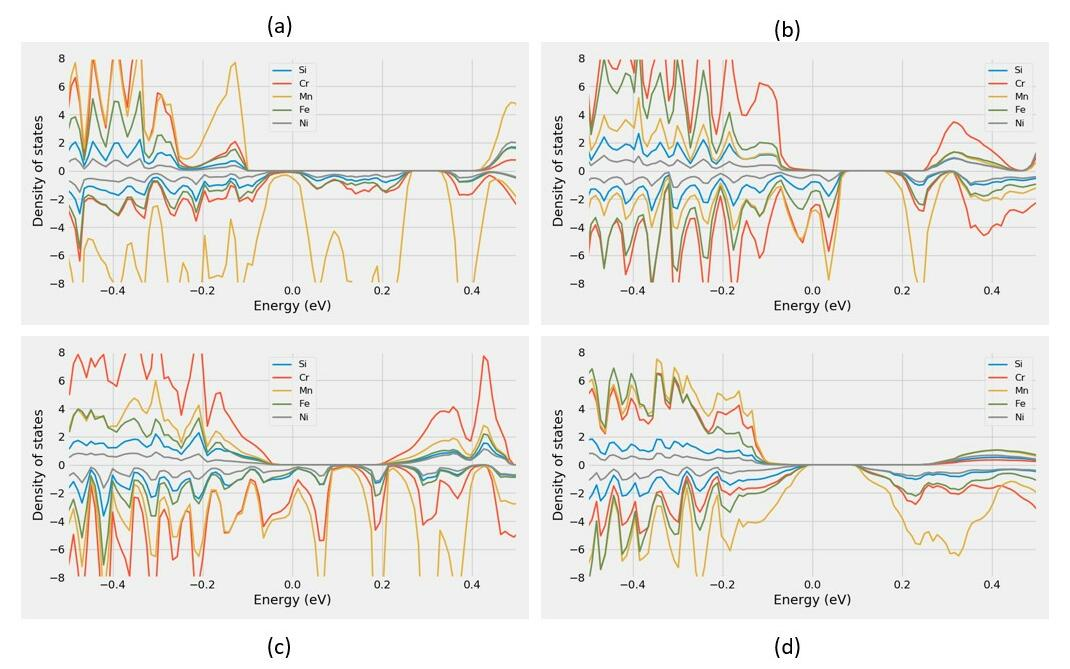
\includegraphics[width=\linewidth]{results/fesi2/permutations/perm_LDOS_crop.jpg}
\caption{Projected density of states of (a) \ch{Cr3Fe3Mn7Ni3Si32} (SQS B), (b) \ch{Cr5Fe5Mn3Ni3Si32} (SQS C), (c) \ch{Cr5Fe3Mn5Ni3Si32} (SQS A), (d) \ch{Cr3Fe5Mn5Ni3Si32} (SQS D)}
\end{figure}

With that said, the plotted PDOSs in figure 7.1 is in good agreement with the listed values in table 7.2. \ch{Cr3Fe3Mn7Ni3Si32} (7.1 a) and \ch{Cr5Fe3Mn5Ni3Si32} (7.1 c) both indicate a sizable spin up band gap, further figure (7.1 d) point to a total band gap around 0.1 eV for SQS D of \ch{Cr3Fe5Mn5Ni3Si32}. On the other hand we find dissimilarity between the density of \ch{Cr5Fe5Mn3Ni3Si32} SQS C and the eigenvalue band gap listed in table 7.2. In figure 7.1 d we find a range of forbidden energies slightly above the Fermi energy, and very small values in spin up at the Fermi energy. Similar to what we experienced in the 192 atom SQS in section 7.4, the eigenvalues report a finite band despite of defect states. Therefore the density of states is not completely zero at $E_F$. 

\begin{figure}[H]
	\centering
	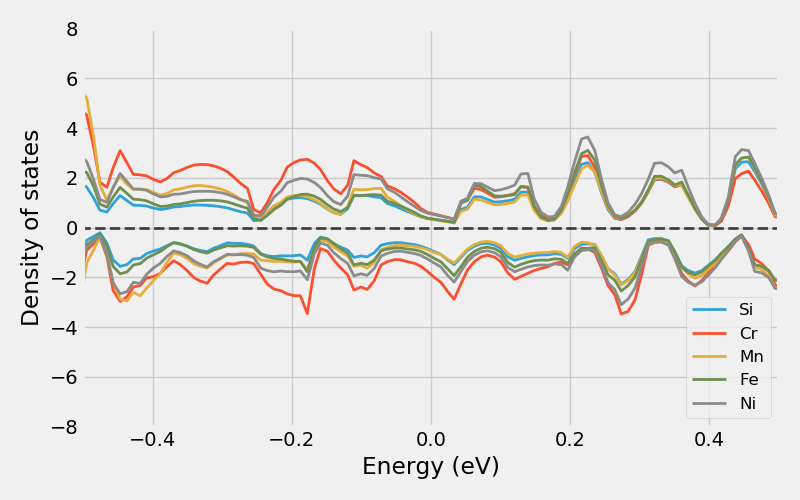
\includegraphics[width=.6\textwidth]{results/fesi2/permutations/ni7_PDOS.png}
	\caption{Projected density of states of \ch{Cr3Fe3Mn3Ni7Si32} around $E_F$}
\end{figure}

In figure 8.6 we saw that electrons from manganese atoms in particular was a key contributor as to why the spin down channel of \ch{(CrFeMnNi)Si2} was metallic in the stable supercell D. This is also largely the case in the permutations shown above in figure 8.12. The proportion of manganese atoms in the alloy seems to offer a very positive effect on the band gap in spin up, but is often detrimental to spin down. This is seen in figure 8.12 (a) and (c) for \ch{Cr3Fe3Mn7Ni3Si32} and \ch{Cr5Fe3Mn5Ni3Si32} respectively, that both contain increased amounts of manganese. By reducing the number of Mn as in (b) we still find that the Mn electrons plague the states at $E_F$ in spin down. In analog we see from (b) and (c) that also Cr negatively impacts to the band gap especially in spin up. The sole permutation with clear evidence of a spin down gap is from the chromium poor permutation plotted in (d). Also in this structure we see that the effects of Mn around $E_F$ is dampened in comparison to the other permutations, despite containing relatively increased amounts of Mn to the eqvimolar alloy.  

An important property of these results is that because each composition alters simultaneous elements, interpreting and relating the results to a particular alteration is challenging. For example, is the result of the \ch{Cr5Fe3Mn5Ni3Si32} permutation a consequence of less Fe or increments to both Cr and Mn? Furthermore is the large band gap in spin up of \ch{Cr3Fe3Mn7Ni3Si32} a product of increasing manganese or reducing the other elements. From the comparatively large gaps in spin up of \ch{Cr3Fe3Mn7Ni3Si32} and \ch{Cr3Fe5Mn5Ni3Si32} and the more present Cr states in spin up in the Cr rich permutations we here conclude that the band gap is related to lessening of chromium, more so than other effects. However we see from both \ch{Cr5Fe5Mn4Ni3Si32} and \ch{Cr3Fe3Mn3Ni7Si32} (figure 8.2) in addition to the manganese rich composition that Mn plays a vital role on the band gap of these structures. It's clear that the \ch{Cr3Fe5Mn5Ni3Si32} alloy manage to strike a balance between 3d elements that results in a specific interplay and correspondingly very promising properties. In addition we see from the enthalpy of formation that the compositions poor in chormium are more stable than the chromium rich compositions. 

\section{High entropy silicides with cobalt and titanium}

In similar fashion to the previous sections, we here begin by presenting the mean and standard deviation of the total energy and magnetization of a set of SQSs corresponding to different high-entropy silicides of the \ch{Fesi2} unit cell. The compositions we have tested are deliberate combinations intended to investigate both the impact of manganese by replacing the element with Co or Ti, and concepts related to HEA theory such as the atomic size effect. Furthermore Co is a very common element in many stable HEA, as seen in section 2.2, thus we include 3 compositions with Co to study the impact on stability and the functional properties. The results of the aforementioned alloys can be seen bellow in table 9.1, note that all compounds contain a total of 48 atoms as before.  

\begin{table}[H]
\centering
\begin{tabular}{@{}cccccc@{}}
\toprule
Composition           & \multicolumn{2}{c}{\begin{tabular}[c]{@{}c@{}}Toten \\ (eV)\end{tabular}} & \multicolumn{2}{c}{\begin{tabular}[c]{@{}c@{}}Mag\\ ($\mu_B$)\end{tabular}} & \begin{tabular}[c]{@{}c@{}}$E_{FPA}$\\ (eV)\end{tabular} \\ \midrule
                      & mean                                 & std                                & mean                                 & std                                  & mean                                                      \\ \midrule
\ch{Cr4Fe4Co4Ni4Si32} & - 6.4655                             & 0.0056                             & 0.0083                               & 0.0155                               & -0.308                                                 \\
\ch{Co4Fe4Mn4Ni4Si32} & - 6.4731                             & 0.0046                             & 0.0000                               & 0.0000                               & -0.355                                                 \\
\ch{Cr4Fe4Ti4Ni4Si32} & - 6.4217                             & 0.0087                             & 0.0305                               & 0.0293                               & -0.209                                                  \\
\ch{Cr4Fe4Mn4Ti4Si32} & -6.6994                              & 0.0071                             & 0.1142                               & 0.0641                               & -0.199                                                  \\
\ch{Cr4Fe4Mn4Co4Si32} & -6.7687                              & 0.0034                             & 0.1331                               & 0.0326                               & -0.323                                                  \\ \bottomrule
\end{tabular}
\caption{Overview new compositions}
\end{table}

From table 9.1 we see that the stability of the relative compositions vary greatly. By introducing cobalt to the alloys, particularly at the cost of chromium result in a large positive effect on the stability, contrary replacing either manganese or nickel with titanium significantly lowers the stability. A physical interpretation of the relative stability is difficult from the overall shallow emphasis and analysis in this project, but we do note that the two most stable alloys consist of the most chemically similar elements in terms of properties such as electronegativity and atomic size. Following the least stable alloys according to our study is comprised of the most chemically dissimilar elements. This is in good agreement with our discussion in section 2.2 regarding phase formation of high-entropy alloys.


In table 9.1 we have listed the mean magnetic moment of the compositions, in line with previous results in this project the magnetization is very dependent on chromium and manganese. This is seen by the overall lowest magnetic moments in the two compositions without these elements, and reversely the highest magnetic moments is found for compositions with both Cr and Mn. Comparing the magnetic moment of \ch{(CrFeCoNi)Si2} and \ch{(CoFeMnNi)Si2} it seems in our study that chromium is most responsible for the magnetic moment in these alloys. Furthermore we find that substituting Ni with both Ti and Co result in more magnetic compounds. These are truly surprising results, one would expect that the magnetic moments would be larger in the ferromagnetic elements Ni, Fe and Co than Cr, Mn and ti. This could go back to our simplistic and superficial study of the magnetic properties in this project, additionly the PBE functional as we covered in section .. have shown limitations for 3d elements and particularly Ni. Thus this could be a factor affecting our results. Another factor is that we here based our comparison on the mean values between 5 SQSs. As we have experienced throughout this project the unieqeness of the SQSs can be troublesome to handle, and our best guess is to study the most stable super-cell. Bellow in table 9.2 we list the magnetic moments of the most stable SQSs. Here we find several dissimilarities to the mean value such as the \ch{Cr4Fe4Co4Ni4Si32} being nonmagnetic in the most stable supercell. Thus based on the utmost stable configurations we can state that replacing either Cr or Mn (with Co) removes the magnetic moment in the alloy. Furthermore we find from these supercells that the magnetic moment is reduced by replacing Ni with Ti, and increased from Co. These results are in much better accordance with previous knowledge of ferromagnetic elements and their interplay in high-entropy alloys.

\begin{table}[H]
\centering
\begin{tabular}{@{}lc@{}}
\toprule
\multicolumn{1}{c}{Composition} & \begin{tabular}[c]{@{}c@{}}Magnetic moment\\ ($\mu_B$)\end{tabular} \\ \midrule
\ch{Cr4Fe4Co4Ni4Si32}           & 0                                                                   \\
\ch{Co4Fe4Mn4Ni4Si32}           & 0                                                                   \\
\ch{Cr4Fe4Ti4Ni4Si32}           & 0,0653                                                              \\
\ch{Cr4Fe4Mn4Ti4Si32}           & 0,0785                                                              \\
\ch{Cr4Fe4Mn4Co4Si32}           & 0,1666                                                              \\ \bottomrule
\end{tabular}
\caption{Final magnetic moment of the most stable supercell of each composition.}
\end{table}

In regards to the band gap of these compositions, we find most to be metals. The band gap of the most stable SQS of each composition is listed in table 4.3, where we calculate the band gap from the eigenvalues at different occupancy cutoffs. As before the 0 band-gap is caused by defect states in the band gap. By increasing the criteria, in other words only consider states with occupancy above a certain threshold, the band gap become finite at $occ = 0.1$ and converge to around $0.02 - 0.06$ eV depending on composition, when only considering full/empty states.  

\begin{table}[H]
\centering
\begin{tabular}{@{}ccccc@{}}
\toprule
\multicolumn{1}{l}{Composition}                   & $occ$                     & \begin{tabular}[c]{@{}c@{}}$E_\text{G} ^\text{up, eigen}$\\ (eV)\end{tabular} & \begin{tabular}[c]{@{}c@{}}$E_\text{G} ^\text{dw, eigen}$\\ (eV)\end{tabular} & \begin{tabular}[c]{@{}c@{}}$E_\text{G} ^\text{tot, eigen}$\\ (eV)\end{tabular} \\ \midrule
\multicolumn{1}{c|}{\multirow{3}{*}{\ch{CrFeCoNiSi2}}}                  & \multicolumn{1}{c|}{0.5}  & 0                                                                             & 0                                                                             & 0                                                                              \\
\multicolumn{1}{c|}{}                             & \multicolumn{1}{c|}{0.1}  & 0.00095                                                                       & 0.0399                                                                        & 0.00095                                                                        \\
\multicolumn{1}{c|}{}                             & \multicolumn{1}{c|}{0.01} & 0.063                                                                         & 0.063                                                                         & 0.063                                                                          \\ \midrule
\multicolumn{1}{c|}{\multirow{3}{*}{\ch{CrFeTiNiSi2}}} & \multicolumn{1}{c|}{0.5}  & 0.0067                                                                        & 0                                                                             & 0                                                                              \\
\multicolumn{1}{c|}{}                             & \multicolumn{1}{c|}{0.1}  & 0.061                                                                         & 0.0087                                                                        & 0.0087                                                                         \\
\multicolumn{1}{c|}{}                             & \multicolumn{1}{c|}{0.01} & 0.061                                                                         & 0.037                                                                         & 0.037                                                                          \\ \midrule
\multicolumn{1}{c|}{\multirow{3}{*}{\ch{CoFeMnNiSi2}}} & \multicolumn{1}{c|}{0.5}  & 0                                                                             & 0                                                                             & 0                                                                              \\
\multicolumn{1}{c|}{}                             & \multicolumn{1}{c|}{0.1}  & 0.0037                                                                        & 0.0037                                                                        & 0.0037                                                                         \\
\multicolumn{1}{c|}{}                             & \multicolumn{1}{c|}{0.01} & 0.0268                                                                        & 0.0268                                                                        & 0.0268                                                                         \\ \midrule
\multicolumn{1}{c|}{\multirow{3}{*}{\ch{CrFeMnTiSi2}}} & \multicolumn{1}{c|}{0.5}  & 0                                                                             & 0                                                                             & 0                                                                              \\
\multicolumn{1}{c|}{}                             & \multicolumn{1}{c|}{0.1}  & 0.021                                                                         & 0.00049                                                                       & 0                                                                              \\
\multicolumn{1}{c|}{}                             & \multicolumn{1}{c|}{0.01} & 0.03                                                                          & 0.03                                                                          & 0.022                                                                          \\ \midrule
\multicolumn{1}{c|}{\multirow{3}{*}{\ch{CrFeMnCoSi2}}} & \multicolumn{1}{c|}{0.5}  & 0.461                                                                         & 0                                                                             & 0                                                                              \\
\multicolumn{1}{c|}{}                             & \multicolumn{1}{c|}{0.1}  & 0.607                                                                         & 0.0218                                                                        & 0.0218                                                                         \\
\multicolumn{1}{c|}{}                             & \multicolumn{1}{c|}{0.01}                      & 0.607                                                                         & 0.0245                                                                        & 0.0245                                                                         \\ \bottomrule
\end{tabular}
\caption{Band gaps of the most stable SQS of $\beta-$ \ch{FeSi2} high-entropy silicide compositions as a function of occupancy in the eigenvalues.}
\end{table}

In the \ch{CrFeMnCoSi2} composition we observe a band gap of around 0.5 eV in the spin up channel, contrary to the metallic or very narrow band gaps in the other compositions. But also in this case we find that the eigenvalues contain defect states, by the fact that the band gap can be enlarged at lower values of $occ$. As we have covered for other examples in this project, this results in a metallic density of states with a small number of states at the Fermi energy. This can be seen from the projected density of states in figure 8.3. This is a contradicting result to the eigenvalues, as per the definition, a band gap is defined as a range of energies around $E_F$ with no states. On the other hand, this result could rather be related to numerical factors affecting the accuracy of the density of states, such as a low resolution or number of k-points considering the very marginal difference separating the density of states from a metal to a half-metal.
  
\begin{figure}[H]
\centering
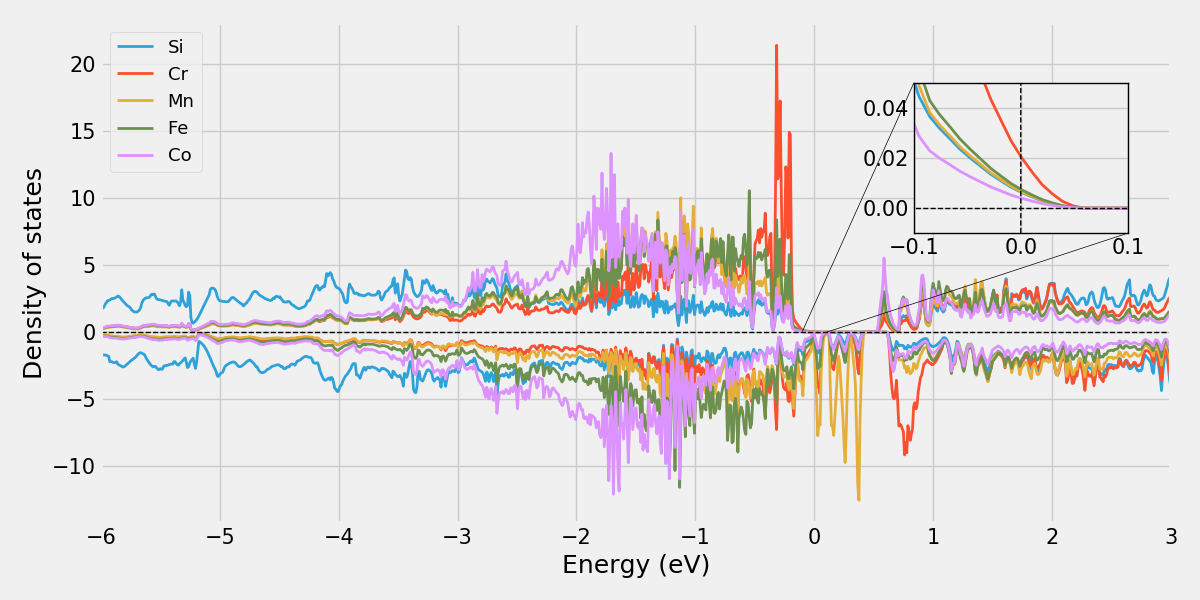
\includegraphics[width=\textwidth]{results/fesi2/composistions/crfemnco_PDOS.png}
\caption{Projected density of states of \ch{(CrFeMnCo)Si2}.}
\end{figure}

The concept of defect states remain as the unsolved biproduct of this project, that we have seen is clearly related to a metallic structure, but is less prominent in the alloys. However considering the scope and allocated time/resources of this project we have not been able to investigate this concept further and found minimal literature to base our results and discussion on. Thus we are unable to provide a conclusion on firstly the significanse and physical interpretation of it, and secondly why they appear in some compositions/structures but not others but report that it's less apparent in the \ch{(CrFeMnNi)Si2} system. One possible method of anlayzing it could have been to study more in depth the pair distribution functions and compare between all compositions, but given the unieqness of the SQSs and number of bonds in each structure this falls outside the scope of this project. We report the related PDF's of each composistion in appendix .. but do not discuss them. The projected density of states of each composition is found in appendix ..

\begin{figure}[H]
\begin{subfigure}{.5\textwidth}
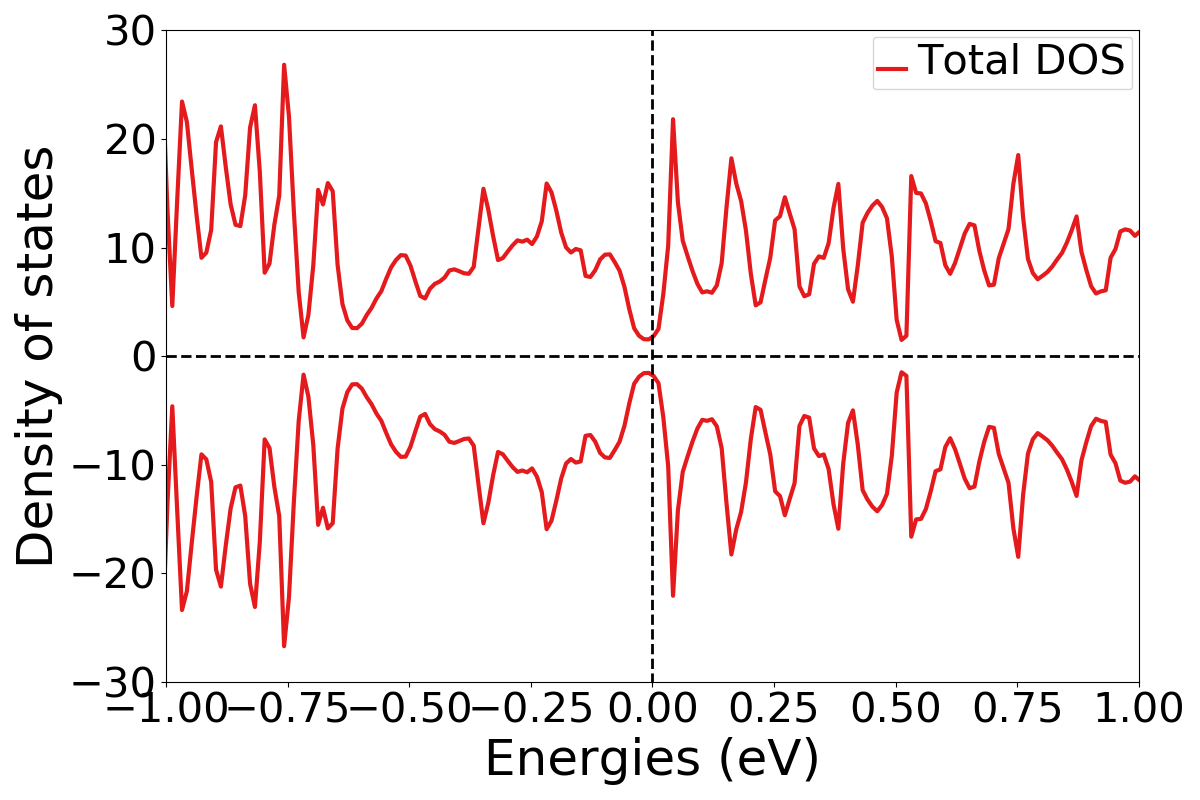
\includegraphics[width=\textwidth]{results/fesi2/composistions/crfeconi_DOS.png}
\caption{\ch{(CrFeCoNi)Si2}}
\end{subfigure}
\begin{subfigure}{.5\textwidth}
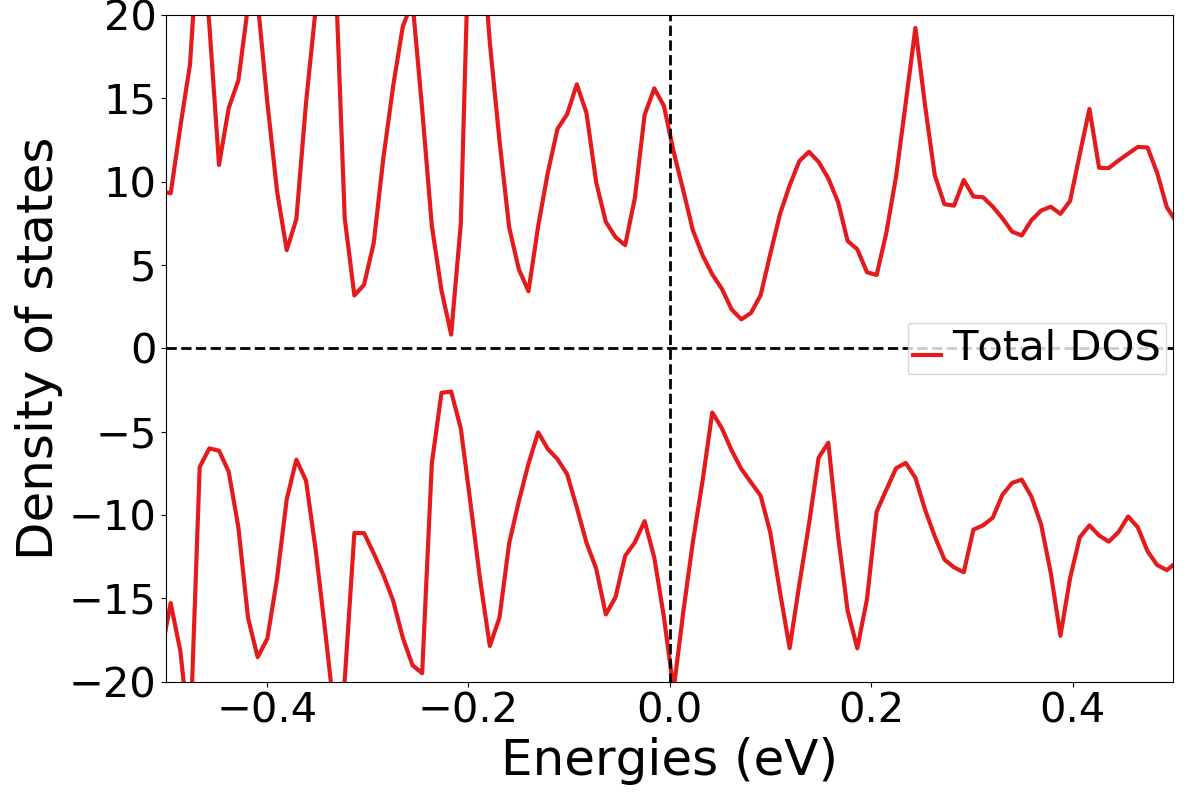
\includegraphics[width=\textwidth]{results/fesi2/composistions/crfetini_DOS.png}
\caption{\ch{(CrFeTiNi)Si2}}
\end{subfigure}
\caption{Density of states of a) \ch{(CrFeCoNi)Si2} and b) \ch{(CrFeTiNi)Si2}.}
\end{figure} 

Contrary to the above case, inserting Co in the place of manganese clearly result in a metallic structure, as seen in the density of states in figure 9.2 a. Replacing Mn with Ti instead we recall from table 9.3 a a very small defect band gap in spin up, however from figure 9.2b we observe that $E_\text{G}^{dos}$ is equal to zero, thus again $E_G ^\text{dos} \neq E_G ^{eigen}$. Comparing the density of states of \ch{(CrFeCoNi)Si2} and \ch{(CrFeTiNi)Si2} the latter is magnetic and the former nonmagnetic, as we discussed previously.

 Above we have looked at the band gap of the most stable SQS of each composition, but as we have experienced in other cases in this project, the properties can vary between SQSs of the same composition. In both \ch{CrFeCoNiSi2} and \ch{CrFeMnTiSi2} we found only metalic supercells with the exception of one SQS in the latter with a very small defect band gap in spin up. Similarly small defect band gaps was observed in two SQSs of \ch{CrFeTiNiSi2} and the rest as metals. In \ch{CrFeMnCoSi2} we found a large defect band gap in spin up in the most stable configuration, here we find similar band gaps in two other SQSs as well. The most interesting case was found in \ch{CoFeMnNiSi2} where we observed small total band gaps without defect states in two SQSs, these are seen in figure 9.3. In agreement with the nonmagnetic character of this composition, the DOS is symmetric with respect to spin. 

\begin{figure}[H]
\begin{subfigure}{.5\textwidth}
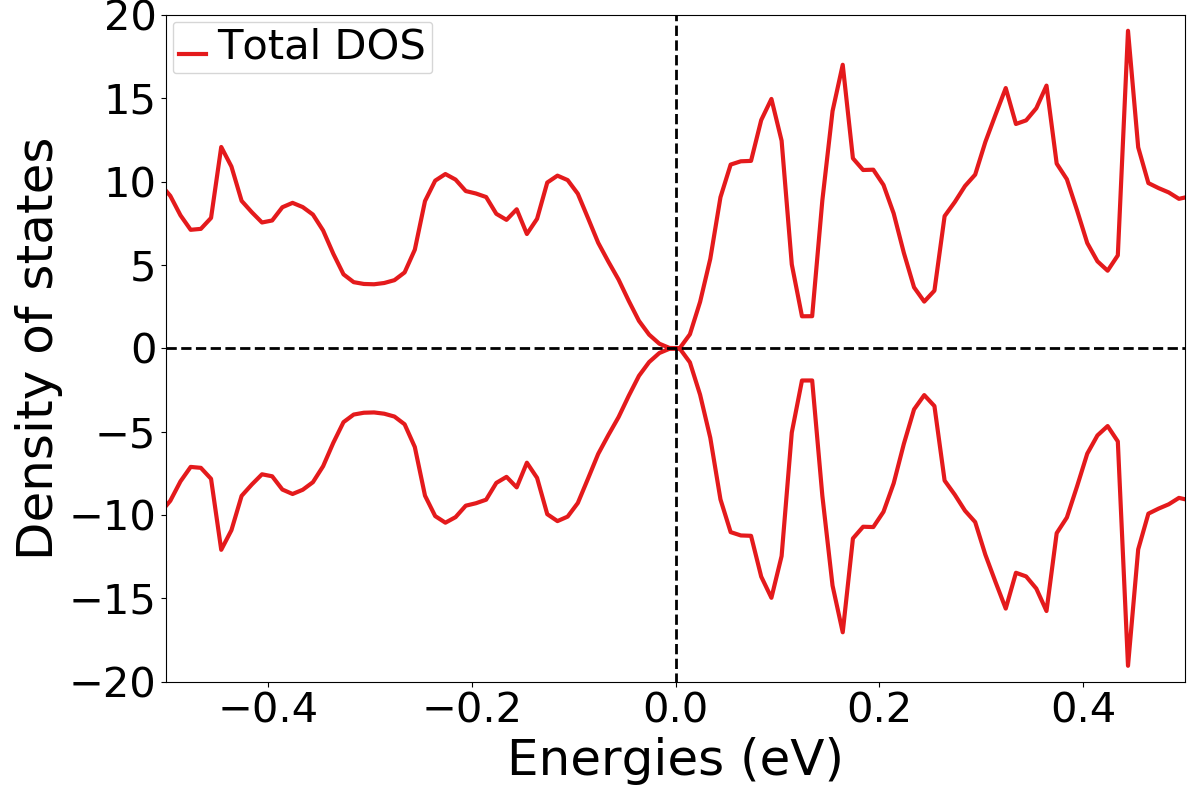
\includegraphics[width=\textwidth]{results/fesi2/composistions/cofemnni_E_DOS.png}
\caption{SQS 1}
\end{subfigure}
\begin{subfigure}{.5\textwidth}
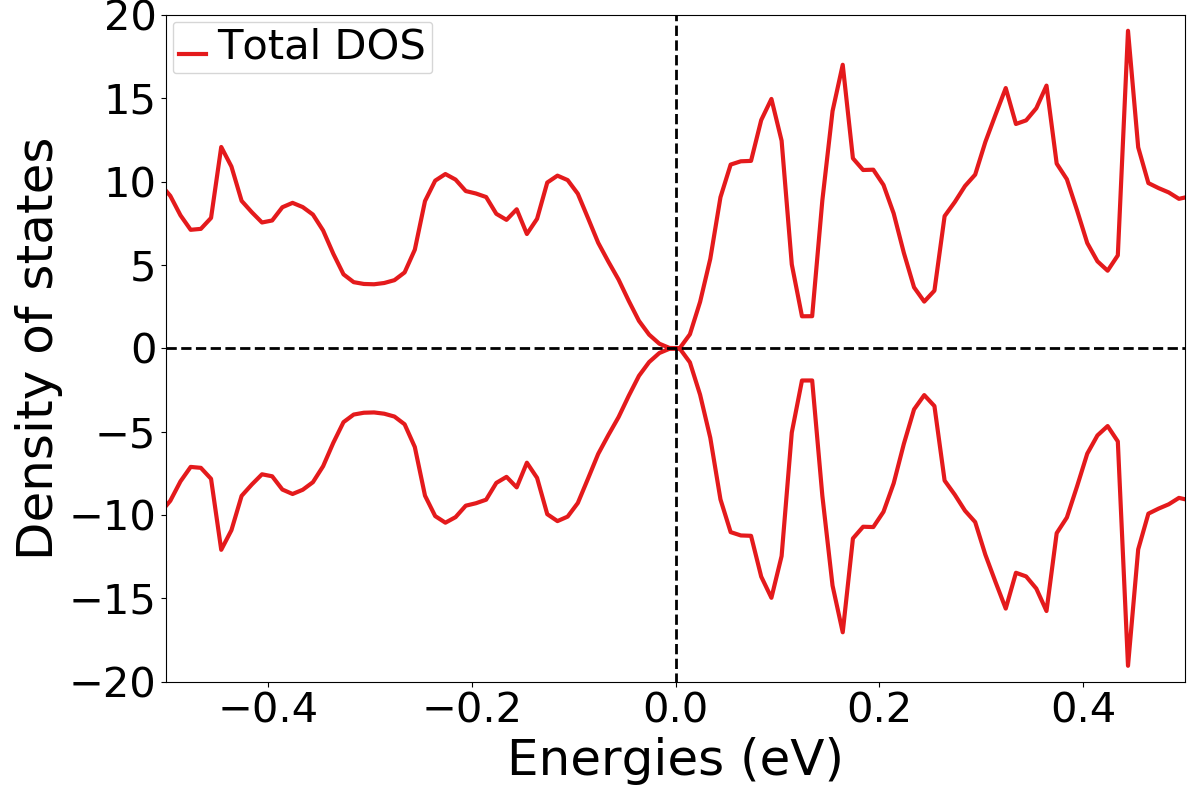
\includegraphics[width=\textwidth]{results/fesi2/composistions/cofemnni_E_DOS.png}
\caption{SQS 2}
\end{subfigure}
\caption{Density of states of two lesser stable SQSs of \ch{(CoFeMnNi)Si2}.}
\end{figure} 

In this example, and also throughout this project we have experienced scenarios where the most stable SQS represents the set of supercells well, and in other instances where the properties change from supercell to supercell. Because of the limited efforts on the magnetism and corresponding stability of the alloys in this project, we chose to include and discuss all 5 SQSs in several cases. This goes back to the topics discussed previously in which one might expect the real material to be comprised of domains of local ordering equal to each one of the SQSs and other possible configuration by a probability based on the relative stability. Furthermore we have reservations about the SQS approach in general to produce an accurate depiction of the true disordered structure, particularly at the relative small size. As we experienced in section .., noteworthy the band gap and PDFs showed distinctions between cells, an additional point to this is that the SQS method have prior limitations of compositions with large deviation from the equiatomic composition, compared to methods such as the CPA for instance.   

Now that we in this study have quite qualitatively determined the existence of a band gap in a potential high-entropy silicides, and according to our calculations in the \ch{(CrFeMnNi)Si2} composition based on the cmce crystal structure. In future work we would first and foremost do a more comprehensive configuration of the magnetic moments to qualitatively determine the ground state energy and compare the relative stability between a broader number of crystal structures. Going back to section 4.3, one of the key drawbacks of the DFT is that we only find local mimina, thus from this project we have no knowledge of this particular composition stabilize in the structure tested in this project or another one. On this topic, recent findings have supported high-entropy silicides stabilizing in less symmetric structures such as orthorombic and hexagonal \textbf{Cite this and that} as opposed to initial studies indicating that HEAs are primarily found in simple cubic lattices. But this should be tested nevertheless. With a more precise conclusion on both geometric and magnetic factors of the material, we could have performed a deeper analysis of the band gap and put more effort into converging calculations without uncertainties of band-gap specialized functionals such as HSE06 and MBJ, and to a greater extent investigated the defect states in the eigenvalues, and relate this qualitatively to a physical or numerical factor.
 
Following studies on the ground state geometry and energy, the composition should be exposed for finite temperatures to evaluate the magnetism and transition temperatures, and entropic contributions to the stability through Gibbs law, in addition to a number of other considerations. Nevertheless we have succeeded atleast within the scope of this project, in our task of locating high-entropy alloys/silicides with a band gap. Furthermore the magnitude of the band gap in many instances (between 0.01 - 0.1 eV), if we assume that the PBE GGA underestimate the band gap between $30\% - 50\%$ would make for promising candidate thermoelectric materials. However to qulitatively state the promise of these compositions as thermoelectrics one would have to investigate properties such as the Seebeck coefficient in addition to the electrical and thermal conductivity. But based on the findings of similar materials to the one in this project, such as .. that found lowered thermal conductivity in .. and ,.. in this and that, the possiblity of an effective thermoelectric material is not beyond hope. In addition the strong magnetism and spin polarization of the band gap displayed in this material (according to our narrow study) makes it a promising candidate for spintronics application. 


\textbf{Do the magnetic discussion here or some other place where I summarize the magnetic findings and relate to other studies. Discuss why Fe and Ni for instance is low and Mn and Cr high.}
We find this to be somewhat of a strange result, in agreement with prior conceptions of the magnetism in various 3d transition metals we find from individual calculations of the base elements in their stable configuration under exact conditions as the SQSs, that Fe display the most pronounced magnetic moment, followed by nickel, while both manganese and Cr are nonmagnetic. Source for Mn

 